\documentclass[../../main.tex]{subfiles}

\begin{document}


The component diagram below presents a general view of the application.  The image describes the application  components with the highest level of detail,  as developers will have to implement the business logic  themselves.  The  other  nodes  in  the  system,  as  well  as  the  services,  are  depicted  more  abstractly. The main components are the database management, model, controller and view. 


\begin{figure}[H]
    \centering
    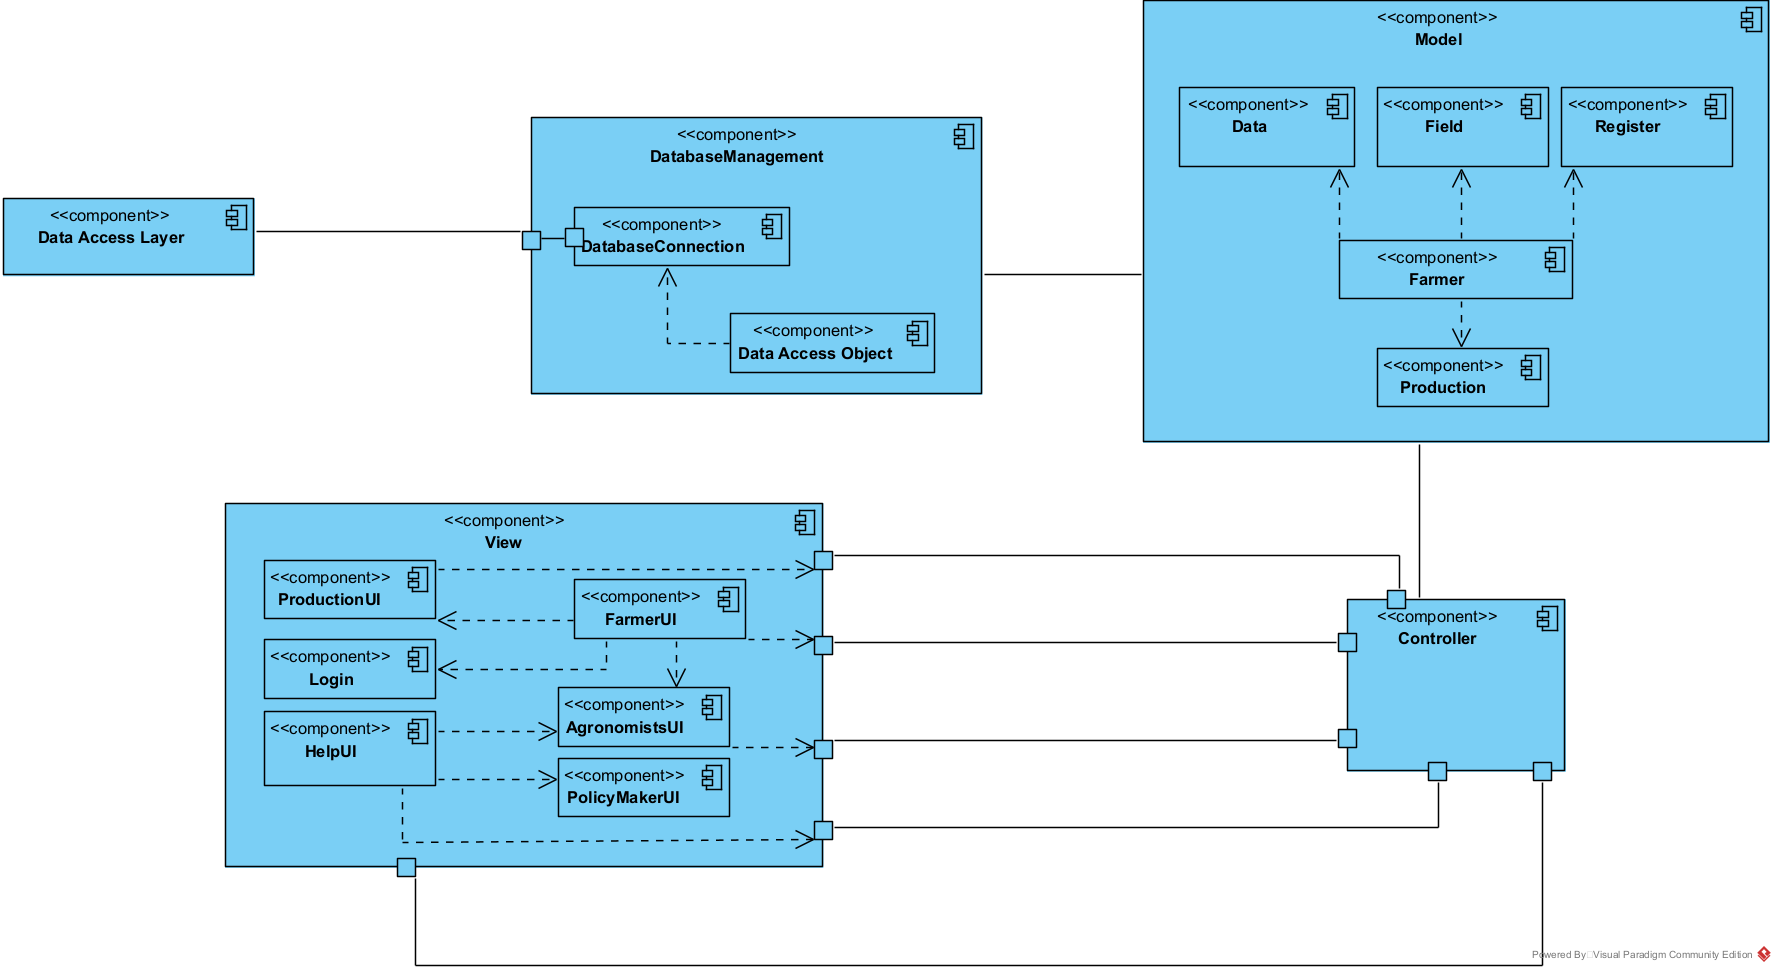
\includegraphics[width=\textwidth]{Component.png}
    \caption{
        Component diagram
    }
\end{figure}


\begin{description}
    
    \item[Farmers] Register with personal data, upload produce information and production, get help in the app, and post questions in the forum. Farmers use the system to get weather information for their current location and to
get advice on planting crops. Farmers can also create discussion forums like a forum where they can upload their current problems in the system. 

    \item[Agronomists] Register with areas of responsibility and help farmers who are facing problems. Agronomists can answer farmers’ questions and get the current weather data of the region and the best 
performing farmers in the system. They can also access local farmers according to the daily plan and update 
the daily plan daily.


    \item[Telengana’s policy makers]  Register as an administrator and have access to view detailed data on farmer production and farmers who have been helped. Telengana’s policy makers have access to the farmer performance rankings in the DREAM system to distinguish between farmers who are performing well and those who are not. The effectiveness of the policy is determined by comparing the ranking of the badly performing farmers over time.
  
  
  
\end{description}

\end{document}
